\documentclass[crop,tikz]{standalone}

\usepackage{fontspec}
\setmainfont{texgyrepagella}[
  Extension = .otf,
  UprightFont = *-regular,
  BoldFont = *-bold,
  ItalicFont = *-italic,
  BoldItalicFont = *-bolditalic,
]

\usepackage{tikz}
\usetikzlibrary{decorations.pathreplacing,calligraphy}
\usetikzlibrary{calc}

\makeatletter % https://tex.stackexchange.com/a/38995/121799
\tikzset{
  use path/.code={\pgfsyssoftpath@setcurrentpath{#1}}
}
\makeatother
\tikzset{reverseclip/.style={insert path={(current bounding box.north
        east) rectangle (current bounding box.south west)}}}

\pgfdeclarelayer{bg}
\pgfsetlayers{bg,main}


\begin{document}
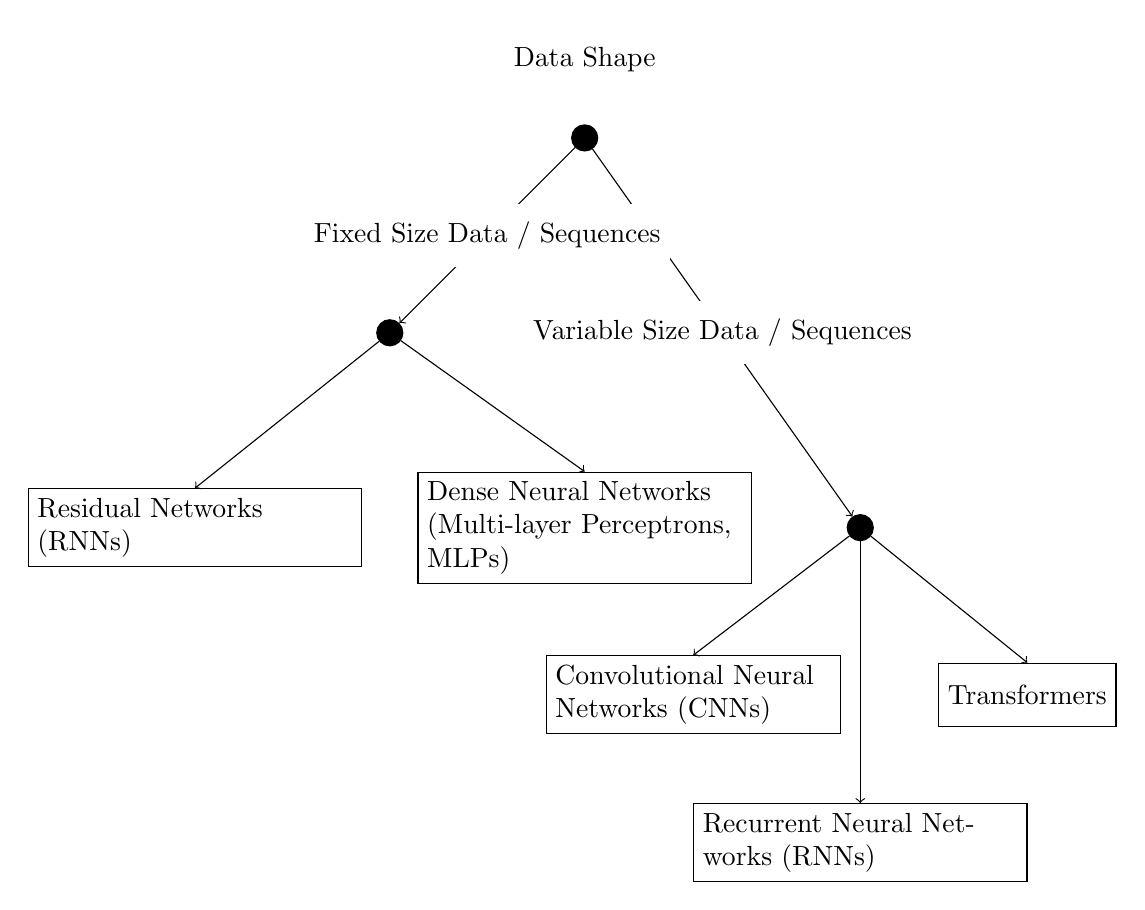
\begin{tikzpicture}
    \tikzstyle{every node}=[node distance=3.5cm,minimum height=0.8cm]
    % data shape
    \node[draw,fill=black,minimum height=0.2cm,circle] (taskroot) at (0,0) {};
    \node[above of=taskroot, node distance=1cm] {Data Shape};

    % fixed input shape
    \node[draw,fill=black,minimum height=0.2cm,circle, below left of=taskroot] (fixed)  {};

    % ResNet
    \node[draw, below left of=fixed,text width=4cm] (resnet)  {Residual Networks (RNNs)};
    \draw[->] (fixed) -- (resnet.north);

    % MLP
    \node[draw, below right of=fixed,text width=4cm] (mlp) {Dense Neural Networks (Multi-layer Perceptrons, MLPs)};
    \draw[->] (fixed) -- (mlp.north);

    % sequence
    \node[draw,fill=black,minimum height=0.2cm,circle,right of=mlp] (sequence) {};
    \draw[->] (taskroot) -- node[fill=white] {Variable Size Data / Sequences} (sequence);

    % this here to draw over above line
    \draw[->] (taskroot) -- node[fill=white] {Fixed Size Data / Sequences} (fixed);

    % CNN
    \node[draw, below left of=sequence,text width=3.5cm, node distance=3cm] (cnn) {Convolutional Neural Networks (CNNs)};
    \draw[->] (sequence) -- (cnn.north);

    % RNN
    \node[draw,below of=sequence,text width=4cm, node distance=4cm] (rnn) {Recurrent Neural Networks (RNNs)};
    \draw[->] (sequence) -- (rnn.north);

    % Transformer
    \node[draw,below right of=sequence, node distance=3cm] (transformer) {Transformers};
    \draw[->] (sequence) -- (transformer.north);

\end{tikzpicture}
\end{document}
